\documentclass[aspectratio=169]{beamer}
\usetheme{Darmstadt}
\usepackage[utf8]{inputenc}
\usepackage[normalem]{ulem}
\usepackage{algorithm}
\usepackage{algpseudocode}
\usepackage{minted} 
\usepackage{hyperref}
\usepackage[russian]{babel}
\title{Многозадачное обучение языковых моделей, основанных на механизме внутреннего внимания}
\author{Погорельцев С. А., н.р. Полякова И. Н.}
\institute{МГУ им. Ломоносова, ф-т ВМК, каф. АЯ}
\date{2022}


\begin{document}

\frame{\titlepage}

\section[Многозадачное обучение]{}
 
\begin{frame}
	\frametitle{Многозадачное обучение}
	\textbf{Многозадачное обучение} (MultiTask Learning) - подполе машинного обучения, в котором одновременно решаются несколько задач, при этом используются общие черты и различия между задачами. Это может привести к повышению эффективности обучения и точности прогнозирования для моделей, специфичных для конкретных задач, по сравнению с отдельным обучением моделей.
\end{frame}

\begin{frame}
	\frametitle{Языковые модели, основанные на механизме внутреннего внимания}
	Да да, я про Трансфоремеры и в частности BERT-подобные модели
	\begin{columns}
				\begin{column}{0.2\textwidth}
			\begin{figure}
	       		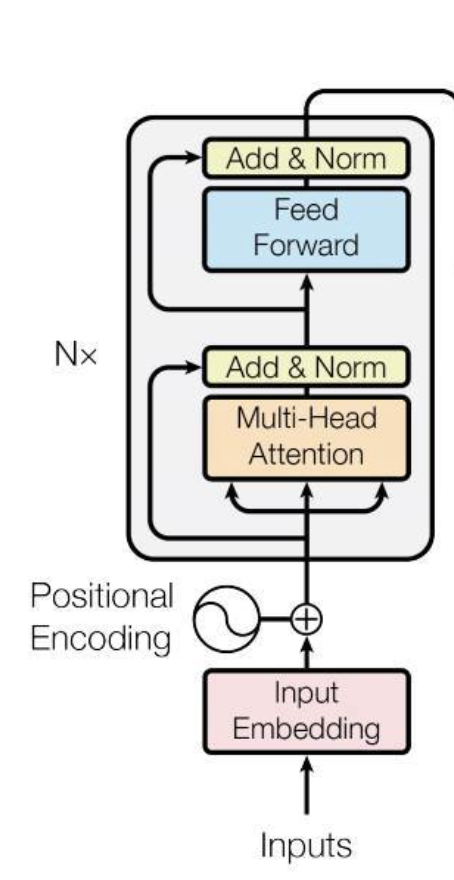
\includegraphics[width=1\textwidth]{assets/trf_enc.png}
	    	\end{figure}
		\end{column}
				\begin{column}{0.8\textwidth}
			\begin{figure}
	       		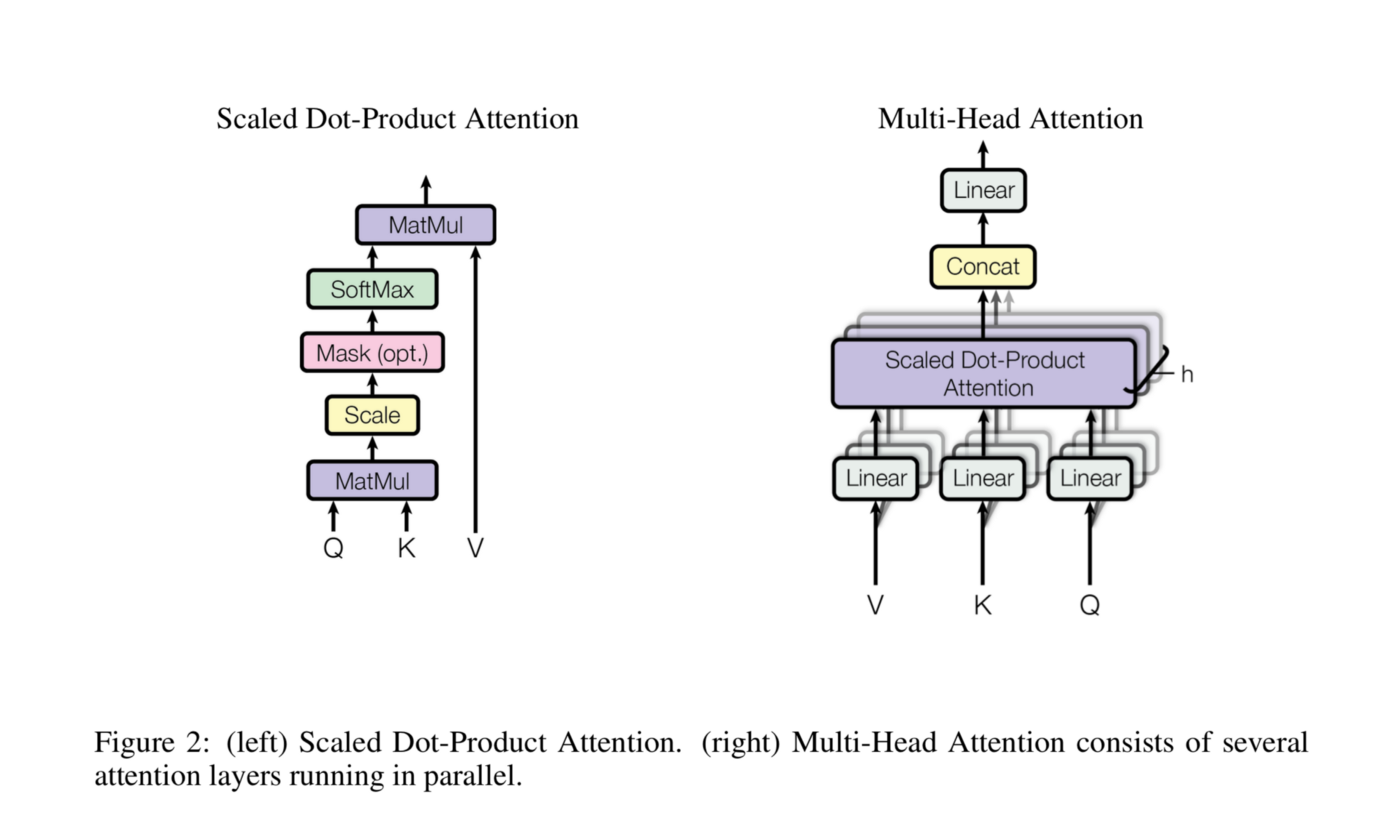
\includegraphics[width=1\textwidth]{assets/mha.png} 
	    	\end{figure}
		\end{column}
	\end{columns}
\end{frame}

\begin{frame}
	\frametitle{Формализация понятия задача}
	\begin{equation}
		T_i = \{p_i(x), p_i(y | x), L_i\}
	\end{equation}
	\begin{itemize}
		\item $p_i(x)$ - распределение входных данных
		\item $p_i(y | x)$ - распределение меток (классификация) / значений (регрессии) в зависимости от входных данных
		\item $L_i$ - функция потерь
	\end{itemize}
	Выборки для задачи
	\begin{itemize}
		\item $D_i^{\opreatorname{train}}$ - обучающая
		\item $D_i^{\opreatorname{val}}$ - валидационная
		\item $D_i^{\opreatorname{test}}$ - тестовая
	\end{itemize}
\end{frame}

\begin{frame}
\frametitle{Гипотезы многозадачной модели (Hard Parameter Sharing)}
Основной вопрос: \textbf{Как огранизовать "переключение"\ на уровне модели?}
\begin{itemize}
	\item Конкатенация one-hot вектора задачи к скрытому представлению
	\begin{figure}
       	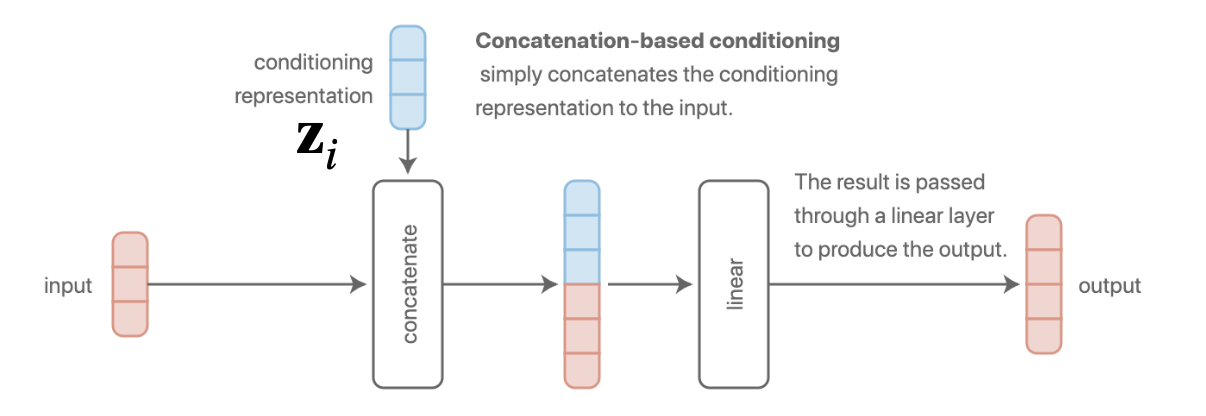
\includegraphics[width=0.8\textwidth]{assets/cat_based_cond.png}
    \end{figure}
	\item Добавление вектора смещения - смещение данных задачи
	\item Умножение - изменение масштаба данных задачи
	\item Архитектура с несколькими головами (популярна, хорошо работает на практике, в дальнейшем буду говорить о ней, т. к. использую её в работе)
\end{itemize}
\end{frame}

\begin{frame}
	\frametitle{Архитектура с несколькими головами}
	\begin{columns}
		\begin{column}{0.5\textwidth}
			\begin{figure}
	       		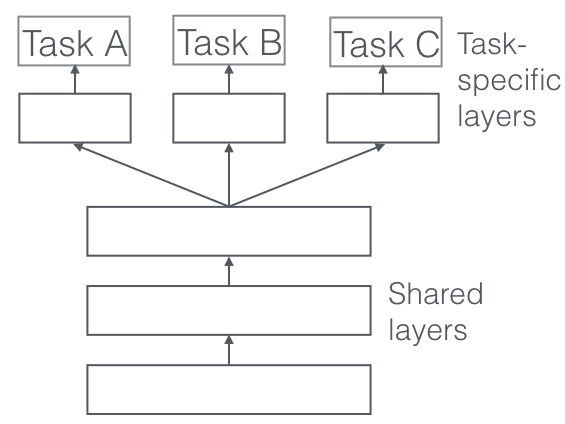
\includegraphics[width=1\textwidth]{assets/multihead_arch.png}
	    	\end{figure}
		\end{column}
		\begin{column}{0.5\textwidth}
			Введём некоторые обозначения и уточним понятие задачи
			\begin{itemize}
				\item $H_i$ - специфичные для задачи слои - голова модели
				\item $E$ - общие слои, формирующие представления для голов $H_i$
			\end{itemize}
			Тогда $i$-ая задача:
			\begin{equation}
				T_i = \{p_i(x), p_i(y | x), H_i, L_i\}
			\end{equation}
			Forward pass для задачи $T_i$
			\begin{equation}
				\opreatorname{F}_i(x) = H_i \circ E \circ x = H_i(E(x))
			\end{equation}
		\end{column}
	\end{columns}
\end{frame}

\begin{frame}
	\frametitle{Обучение многоголовой модели (популярные подходы)}
	\begin{itemize}
		\item \textbf{Одна задача на батч} Данные всех задач разбиваются на батчи и эти батчи перемешиваются вместе. На каждой эпохе выбирается случайный $j$-ый батч соотвествующий задаче $T_i$ $\opreatorname{batch}_j^i$, а затем всё (почти) как обычно.
		\item \textbf{Оптимизация (взвешенной) суммы функций потерь} 
			\begin{itemize}
				\item Собираются "метабатчи"\ $\{ \operatorname{batch}^{1}_{j_1}, \operatorname{batch}^{2}_{j_2}, ..., \operatorname{batch}^{n}_{j_n} \}$ - множество по 1 случайному батчу для каждой задачи (здесь $n$ штук). 
				\item Для каждой $i$-ой задачи вычисляется $\opreatorname{fwd}_i = F_i(\operatorname{batch}^{i}_{j_i}), \opreatorname{loss}_i = L_i(f_i)$ и оптимизируется $loss = \sum_{i = 1}^{n} w_i \operatorname{loss}_i$, где $\forall i \text{ } w_i > 0$.
				\item $w_i$ регулирует важность $i$-ой задачи при оптимизации
			\end{itemize}
	\end{itemize}
	Я экспериментирую с обоими и кажется, что оптимизация суммы работает лучше \sout{что в целом логично, т. к. первый вариант с точки зрения метоптов - тихий ужас}
\end{frame}

\begin{frame}
	\frametitle{Алгоритм обучения с оптимизацией по одной задаче}
	\begin{algorithmic}
		\For {$\operatorname{epochNum} \gets \overline{0, N} $}
			\ForAll {$\operatorname{batch}^{i}_{j} \in \operatoname{batches.shuffle}() $}
				\State $\operatoname{outputs} \gets F_i(batch^{i}_{j})$
				\State $\operatorname{loss} \gets L_i(\operatoname{outputs})$
				\State $\operatorname{F_i} \gets \operatorname{F_i} - \alpha \nabla \operatorname{loss}$ \Comment{Тут может быть любой метод оптимизации}
			\EndFor
		\EndFor
	\end{algorithmic}
	Minibatch градиентный спуск здесь для упрощения примера, чаще используется Adam или AdamW для обучения Трансформеров (в т.ч. многозадачных)
\end{frame}

\begin{frame}
	\frametitle{Алгоритм обучения с оптимизацией по сумме функций потерь}
	\begin{algorithmic}
		\For {$\operatorname{epochNum} \gets \overline{0, N} $} \Comment{Итерация по эпохам}
			\ForAll {$\operatorname{metabatch}_{j} \in \operatoname{metabatches.shuffle}() $}  \Comment{Итерация по "метабатчам"}
				\State $\operatorname{loss} \gets 0$
				\ForAll {$\operatorname{batch}^{i}_{j} \in \operatorname{metabatch}_{j}$} \Comment{Итерация по задачам и их батчам}
					\State $\operatoname{outputs}^{i}_{j} \gets F_i(\operatorname{batch}^{i}_{j})$
					\State $\operatoname{loss}_j \gets \operatoname{loss}_j + w_i L_i(\operatoname{outputs}^{i}_{j}) $
				\EndFor
				% \State $\operatorname{F_i} \gets \operatorname{F_i} - \alpha \nabla \operatorname{loss}$ \Comment{Тут может быть любой метод оптимизации}
				% \State Подумать шо здесь (посмотреть что делает торч)
				\State loss_j.backward(); optimizer.step(); optimizer.zero\_grad() \Comment{*}
			\EndFor
		\EndFor
	\end{algorithmic}
	*: магия автоматического дифференцирования PyTorch, а на самом деле
	\begin{equation*}
		\nabla loss_j(x^{i, j}) = \nabla \sum_{i = 1}^{n} w_i L_i(H_i(E(x^{i, j})) \text{ (продолжение на след. слайде)}
	\end{equation*}
	% Minibatch градиентный спуск здесь для упрощения примера, чаще используется Adam или AdamW для обучения Трансформеров (в т.ч. многозадачных)
\end{frame}

\begin{frame}
	\frametitle{Подробнее про обновление весов для суммы}
	Рассмотрим частную производную для $k$-ой координате
	\begin{equation*}
		(\nabla loss_j (x^{i, j}))_k = \frac{\partial}{\partial x^{i, j}_k} \sum_{i = 1}^{n} w_i L_i(H_i(E(x^{i, j})) = \sum_{i = 1}^{n} w_i \frac{\partial L_i(H_i(E(x^{i, j}))}{\partial x^{i, j}_k}
	\end{equation*}
	Дальше считается как обычно, как и в предыдущем случае градиент от конкретной функции потерь с использованием правила цепочки $\frac{\partial y}{\partial x} = \frac{\partial y}{\partial z} \frac{\partial z}{\partial x}$

	После вычисления градиента делается шаг метода оптимизации обновляются все веса и для общих слоёв, и для \textbf{каждой головы} (backpropagation)

	\begin{itemize}
		\item Полученный метод - обобщение первого (если $w$ - one-hot вектор, то получаем первый метод буквально)
		\item Снижается проблема забывания, поскольку оптимизация всего сразу
		\item Возможно, стоит совместить первый и второй подходы
		\begin{itemize}
			\item Сначала сделать базовую оптимизацию для всех задач
			\item Затем заниматься более тонкой настройкой позадачных весов
		\end{itemize}
	\end{itemize}
\end{frame}

\begin{frame}
\frametitle{Некоторые важные особенности}
\begin{itemize}
	\item \textbf{Transfer Learning}: знания для одной задачи помогают в решении другой
	\item \textbf{Representation Learning}: перенос знаний часто связан с выучиванием общими слоями хороших векторных представлений входных признаков
	\item \textbf{Регуляризация}: многозадачное обучение работает как регуляризация и в случае переобучения всегда можно добавить задач для улучшения генерализации или сделать общими больше слоёв
	\item \textbf{Эффективное использование}: модель одна, пусть и крупнее
\end{itemize}
Сложности
\begin{itemize}
	\item \textbf{Negative Transfer}: бывает, что задачи отрицательно влияют на решение друг друга. Наиболее вероятные причины:
	\begin{itemize}
		\item Недостаточно выразительная модель (часто многозадачные модели больше)
		\item Сложности с оптимизацией (межзадачная интерференция, задачи могут обучаться с разной скоростью)
	\end{itemize}
	\item \textbf{Совместность задач}: какие задачи будут хорошо работать вместе? На этот вопрос ответ пока можно искать только экспериментами (за 1 эпоху понятно)
\end{itemize}
\end{frame}

\section[Разработка модуля]{}

\begin{frame}
	\frametitle{Проблема со средствами многозадачного обучения}
	Во время первых экспериментов обнаружил, что приходится писать много однообразного и сложного кода, потому, что хороших библиотек для многозадачного обучения Трансформеров пока нет (или я плохо искал)

	В итоге, была разработна (и продолжает развиваться) небольшая библиотека, которая позволяет декларативно описывать задачи и сама собирает модель, готовит данные с учётом многозадачности
	\begin{itemize}
		\item Высокоуровневые готовые конфигурации для типичных задач
		\item "Ручки"\ для низкоуровневой настройки задач
		\item Средства для обучения в обычном цикле PyTorch
		\item Обучение с многозадачным аналогом Trainer (сейчас перерабатывается)
	\end{itemize}
\end{frame}

\subsection{Примеры работы с библиотекой}

\begin{frame}[fragile]
	\frametitle{Пример простой конфигурации задач}
	\begin{minted}{python}
tasks = Tasks([
	SequenceClassificationTask(
	    name="danetqa",
	    dataset_dict=load_dataset(...),
	    preprocessor=Preprocessor([preprocess_danetqa]),
	    tokenizer_config=TokenizerConfig(max_length=512),
	), 
	SequenceClassificationTask(
	    name="headline_cause",
	    num_labels=3,
	    dataset_dict=load_dataset(...),
	    preprocessor=Preprocessor([preprocess_headline_cause]),
	    tokenizer_config=cfg
	)], model_path = "DeepPavlov/rubert-base-cased")
	\end{minted}
\end{frame}

\begin{frame}[fragile]
	\frametitle{Низкоуровневая конфигурация задачи}
	\begin{minted}{python}
Task(
    name = "название задачи (для индексации и логов)",
    head = <объект подкласса torch.nn.Module> | HFHead,
    data = Data(
        dataset_dict = <датасет в формате datasets.DatasetDict>,
        # другое (не обязательно, задано по-умолчанию)
        configured_tokenizer = ConfiguredTokenizer(
            model_path, padding = False, truncation = True, max_length
            ... # другие параметры токенизатора Hugging Face
        ),
        preprocessor = Preprocessor(...),
        columns, # поля, которые нужно приводить к формату PyTorch
        collator_class, collator_config
    )
)
	\end{minted}
\end{frame}

\begin{frame}[fragile]
	\frametitle{Конфигурация головы модели}
	\begin{itemize}
		\item Готовая из \texttt{transformers}
		\begin{minted}[fontsize=\small]{python}
head = HFHead(class_ = AutoModelForSequenceClassification,
              config_params = {"num_labels": 2})
		\end{minted}
		\item Свой \texttt{torch.nn.Module}
		\begin{minted}[fontsize=\small]{python}
class TwoLinears(nn.Module):
    def __init__(self, ...):
        layers = [nn.Linear(768, 2048), F.relu, nn.Linear(768, 2)]
        self.layers = nn.ModuleList(layers)
        self.loss = nn.CrossEntropyLoss()
    def forward(self, encoder_outputs, labels, ...):
        x = encoder_outputs[1]
        for layer in self.layers: x = layer.forward(x)
        return {"logits": x, 
                "loss": self.loss(logits.view(-1, num_labels), 
                                  labels.view(-1))}
head = TwoLinears(...)
		\end{minted}
	\end{itemize}
\end{frame}

\begin{frame}[fragile]
	\frametitle{Обучение с циклом на PyTorch}
	\begin{minted}[fontsize=\small]{python}
train_sampler = MultitaskBatchSampler(tasks.data, "train", batch_size=12)
model = MultitaskModel(encoder_path, tasks.heads)
# ... инициализация метода оптимизации, перенос модели на GPU ...
for epoch_num in range(num_epochs):
  for batch in train_sampler:
    batch.data.to(device)
    outputs = model.forward(batch.name, **batch.data)
    loss = outputs.loss
    print(f"Training loss: {loss} on task {batch.name}")
    loss.backward()
    optimizer.step()
    lr_scheduler.step()
    optimizer.zero_grad()
	\end{minted}
\end{frame}

\subsection{Дополнительная информация}

\begin{frame}
	\frametitle{Готовность и открытый доступ}
	\begin{itemize}
		\item Код в открытом доступе \url{https://github.com/s1m0000n/multitask-transformers}
		\item Буду рад новым контрибьюторам
		\item Нормальное состояние кодовой базы (pylint > 8)
		\item Новые вещи реализуются по мере того, что я использую для ВКР
		\item Если есть идеи, что стоит улучшить / добавить - создавайте Issue
		\item Планируется публикация статьи
	\end{itemize}
\end{frame}


\section[Исследование многозадачных трансформеров]{}

\begin{frame}
	\frametitle{Цели и планы (неформально)}
	\begin{itemize}
		\item Попытаться исправить / уменьшить проблемы оптимизации (важно)
		\item Решение проблемы Negative Transfer усложнением голов (важно)
		\item MTL как средство улучшения качества на малых выборках (важно)
		\begin{itemize}
			\item В первоначальных экспериментах удалось улучшить качество задачи DaNetQA 
			\item Обучалось вместе с задачей NLI с позадачной оптимизацией
			\item Планируется рассмотреть подробнее, после прочих улучшений
		\end{itemize}
		\item Рассмотрение многозадачных трансформеров для русского (как получится)
		\item Попробовать свои силы в соревновании \href{https://russiansuperglue.com/}{\color {blue} Russian SuperGLUE} (если успею)
	\end{itemize}
\end{frame}

\begin{frame}
	\frametitle{Сходимость}
	\begin{columns}
		\begin{column}{0.3\textwidth}
			\begin{figure}
	       		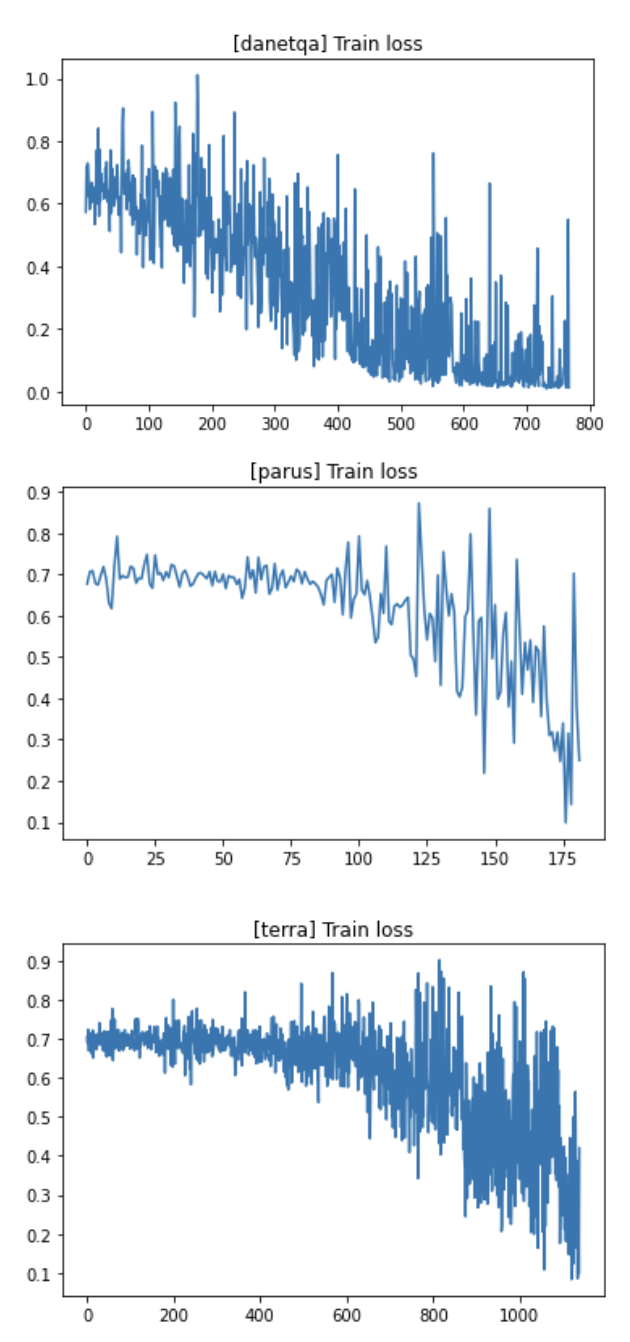
\includegraphics[width=0.7\textwidth]{assets/ttl.png}
	    	\end{figure}
		\end{column}
		\begin{column}{0.7\textwidth}
			\begin{figure}
	       		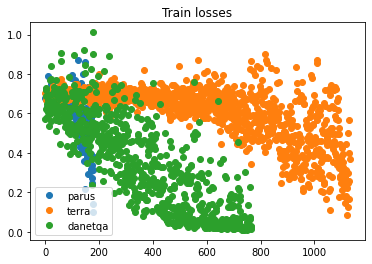
\includegraphics[width=0.8\textwidth]{assets/conv_scatter.png}
	    	\end{figure}
		\end{column}
	\end{columns}
\end{frame}

\begin{frame}
	\frametitle{Анализ первого эксперимента}
	\begin{itemize}
		\item Одновременная сходимость возможна, даже с простым методом оптимизации
		\item Похоже, что с некоторого момента начинается перенос знаний
		\item Задачи с малыми выборками выигрывают от больших “соседей”
		\item Большое внимание стоит уделять оптимизации, например, хорошо работает увеличенное количество шагов разогрева (warmup steps)
	\end{itemize}
\end{frame}


\subsection{Исследование подходов к оптимизации}

\begin{frame}
	\frametitle{Особенности способов оптимизации}
	\begin{itemize}
		\item Обучение с оптимизацией по взвешенной сумме лоссов
		\begin{itemize}
			\item Стабильная сходимость
			\item Грубо оптимизирует всё сразу
			\item Тяжело достичь очень высоких результатов на задачах (согласно метрикам)
			\item Гипотеза: хорошо подойдёт для "грубой"\ и быстрой начальной оптимизации 
		\end{itemize}
		\item Обучение с позадачной оптимизацией
		\begin{itemize}
			\item Медленная и нестабильная сходимость
			\item Наблюдается следующее поведение
			\begin{itemize}
				\item Хорошо пооптимизировал некоторую задачу
				\item Одновременно в разной степени просел на других 
				\item Получаем в целом медленное скачкообразное улучшение лоссов и метрик
			\end{itemize}
			\item Гипотеза: хорошо подойдёт для "тонкой"\ донастройки по задачам, при условии, что проведена начальная "грубая"\ оптимизация
		\end{itemize}
	\end{itemize}
\end{frame}

\begin{frame}
	\frametitle{Предлагаемое улучшение подхода}
	\begin{enumerate}
	  \item Делаем первноначальную оптимизацию: пока не выйдем на плато - обучаемся по взвешенной сумме функций потерь
	  \item Далее - тонкая оптимизация, варианты
	  \begin{itemize}
	  	\item Просто позадачная оптимизация (выше вероятность проблемы забывания)
	  	\item Цикл: N раз выполняем позадачную оптимизацию, а затем один раз по взвешенной сумме (борьба с забыванием)
	  \end{itemize}
	\end{enumerate}
	Так же при первоначальной и точной оптимизациях можно иногда пропускать обучение на задачах, которые по лоссу / метрикам уже оптимизировались значительно лучше, чем остальные

	Это может помочь побороть проблему с разной скоростью сходимости задач

	\textbf{Это пока просто гипотеза, но я её обязательно проверю}
\end{frame}

\begin{frame}
	\frametitle{Экспериментальные наблюдения}
	\begin{itemize}
		\item Обучение с оптимизацией по взвешенной сумме лоссов
		\begin{itemize}
			\item Стабильная сходимость
			\item Грубо оптимизирует всё сразу
		\end{itemize}
		\item Обучение с позадачной оптимизацией
		\begin{itemize}
			\item Медленная и нестабильная сходимость
			\item Наблюдается следующее поведение
			\begin{itemize}
				\item Хорошо пооптимизировал некоторую задачу
				\item Одновременно в разной степени просел на других 
				\item Получаем в целом скачкообразное улучшение лоссов и метрик
			\end{itemize}
		\end{itemize}
	\end{itemize}
\end{frame}

\subsection{Negative Transfer}

\begin{frame}
	\frametitle{Подробнее о проблеме Negative Transfer}
	\begin{columns}
		\begin{column}{0.5\textwidth}
			\begin{figure}
	       		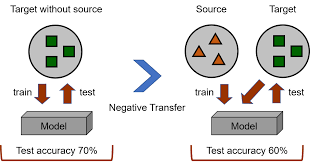
\includegraphics[width=1\textwidth]{assets/nt.png}
	    	\end{figure}
		\end{column}
		\begin{column}{0.5\textwidth}
			\textbf{Основные причины}
			\begin{itemize}
				\item Проблемы оптимизации
				\begin{itemize}
					\item Задачи могут учиться с разной скоростью
					\item Получается слишком сильная регуляризация (регулируем гиперпараметры)
					\item Большой угол между градиентами
				\end{itemize}
				\item Недостаточная выразительность модели - обычно многозадачные модели значительно крупнее, чем однозадачные и требуется \textbf{усложнять гипотезы голов}
			\end{itemize}
		\end{column}
	\end{columns}
\end{frame}

\begin{frame}
	\frametitle{Проблема отличающихся целей}
	\begin{figure}
	    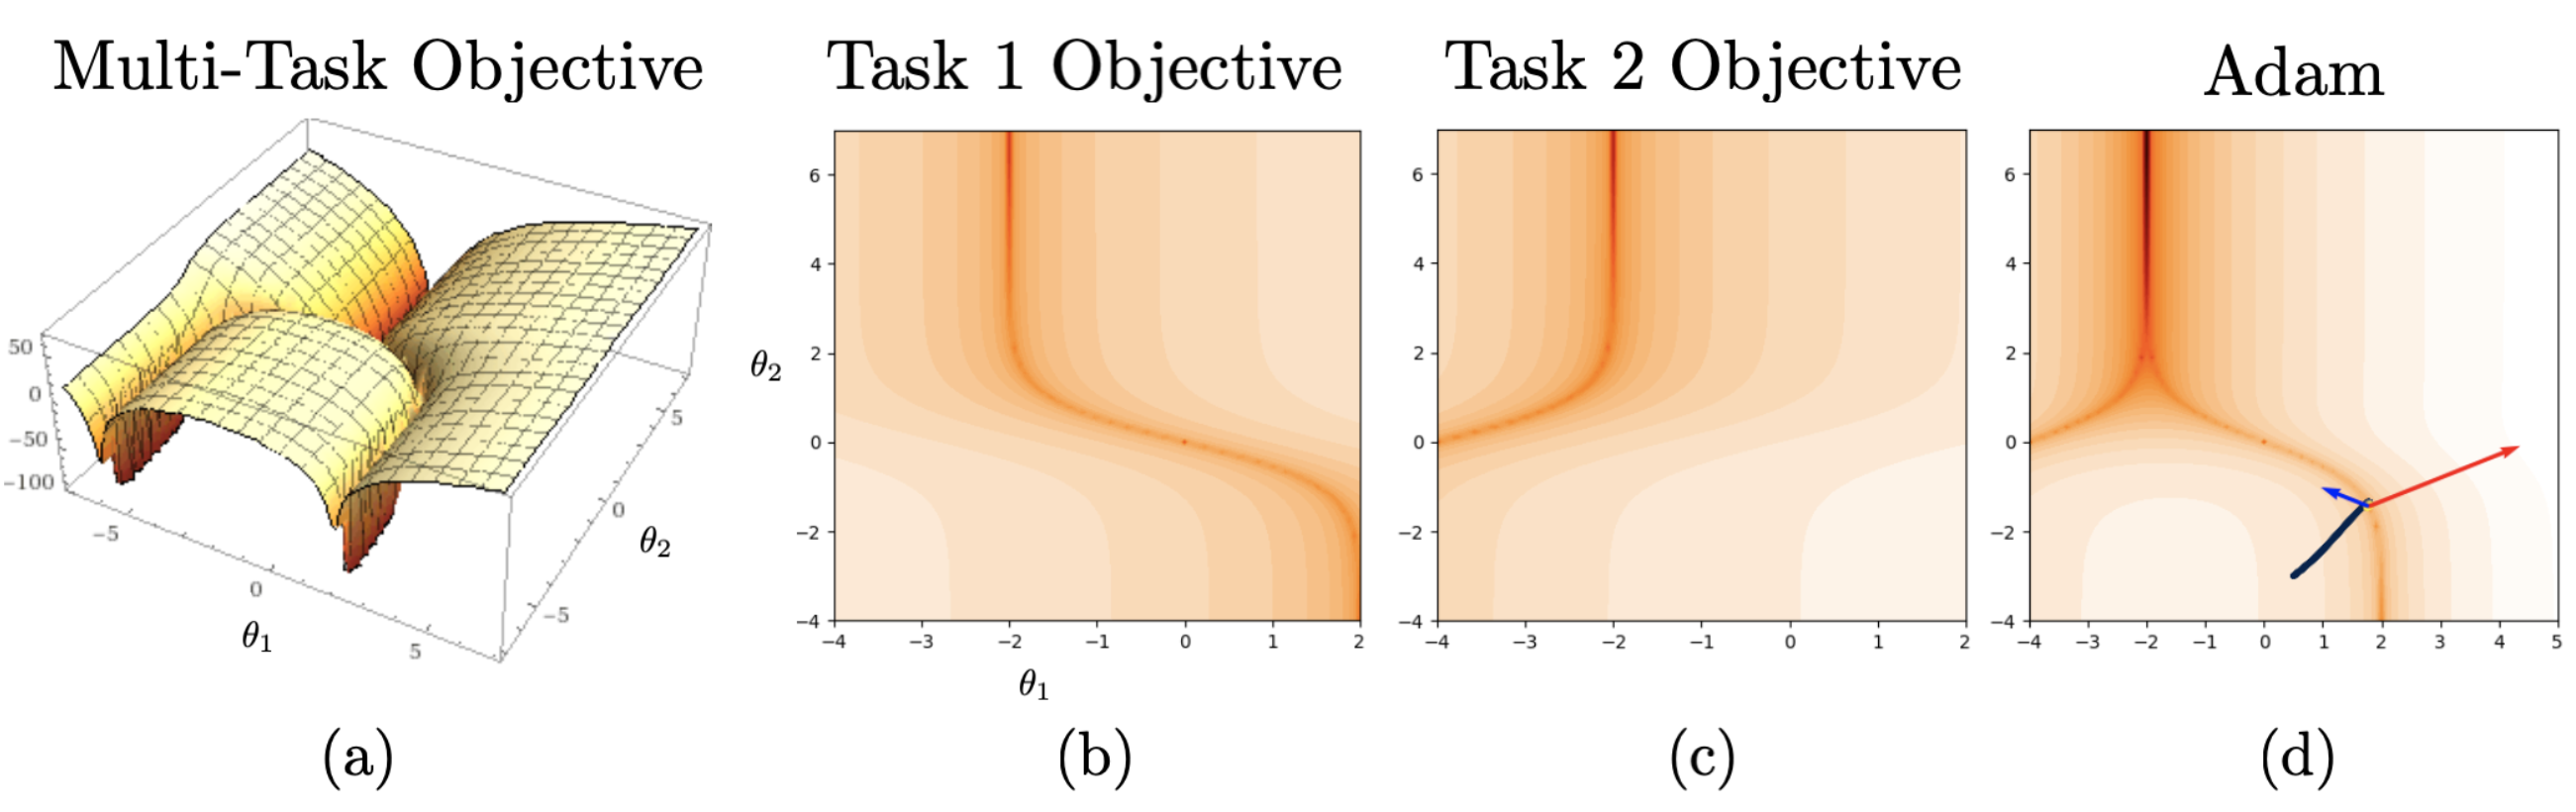
\includegraphics[width=1\textwidth]{assets/grad_angle.png}
	\end{figure}
	\href{https://arxiv.org/abs/2001.06782}{\color {blue} Yu et al. Gradient Surgery for Multi-Task Learning. 2020}
\end{frame}

\begin{frame}
	\frametitle{Решение}
	\begin{figure}
	    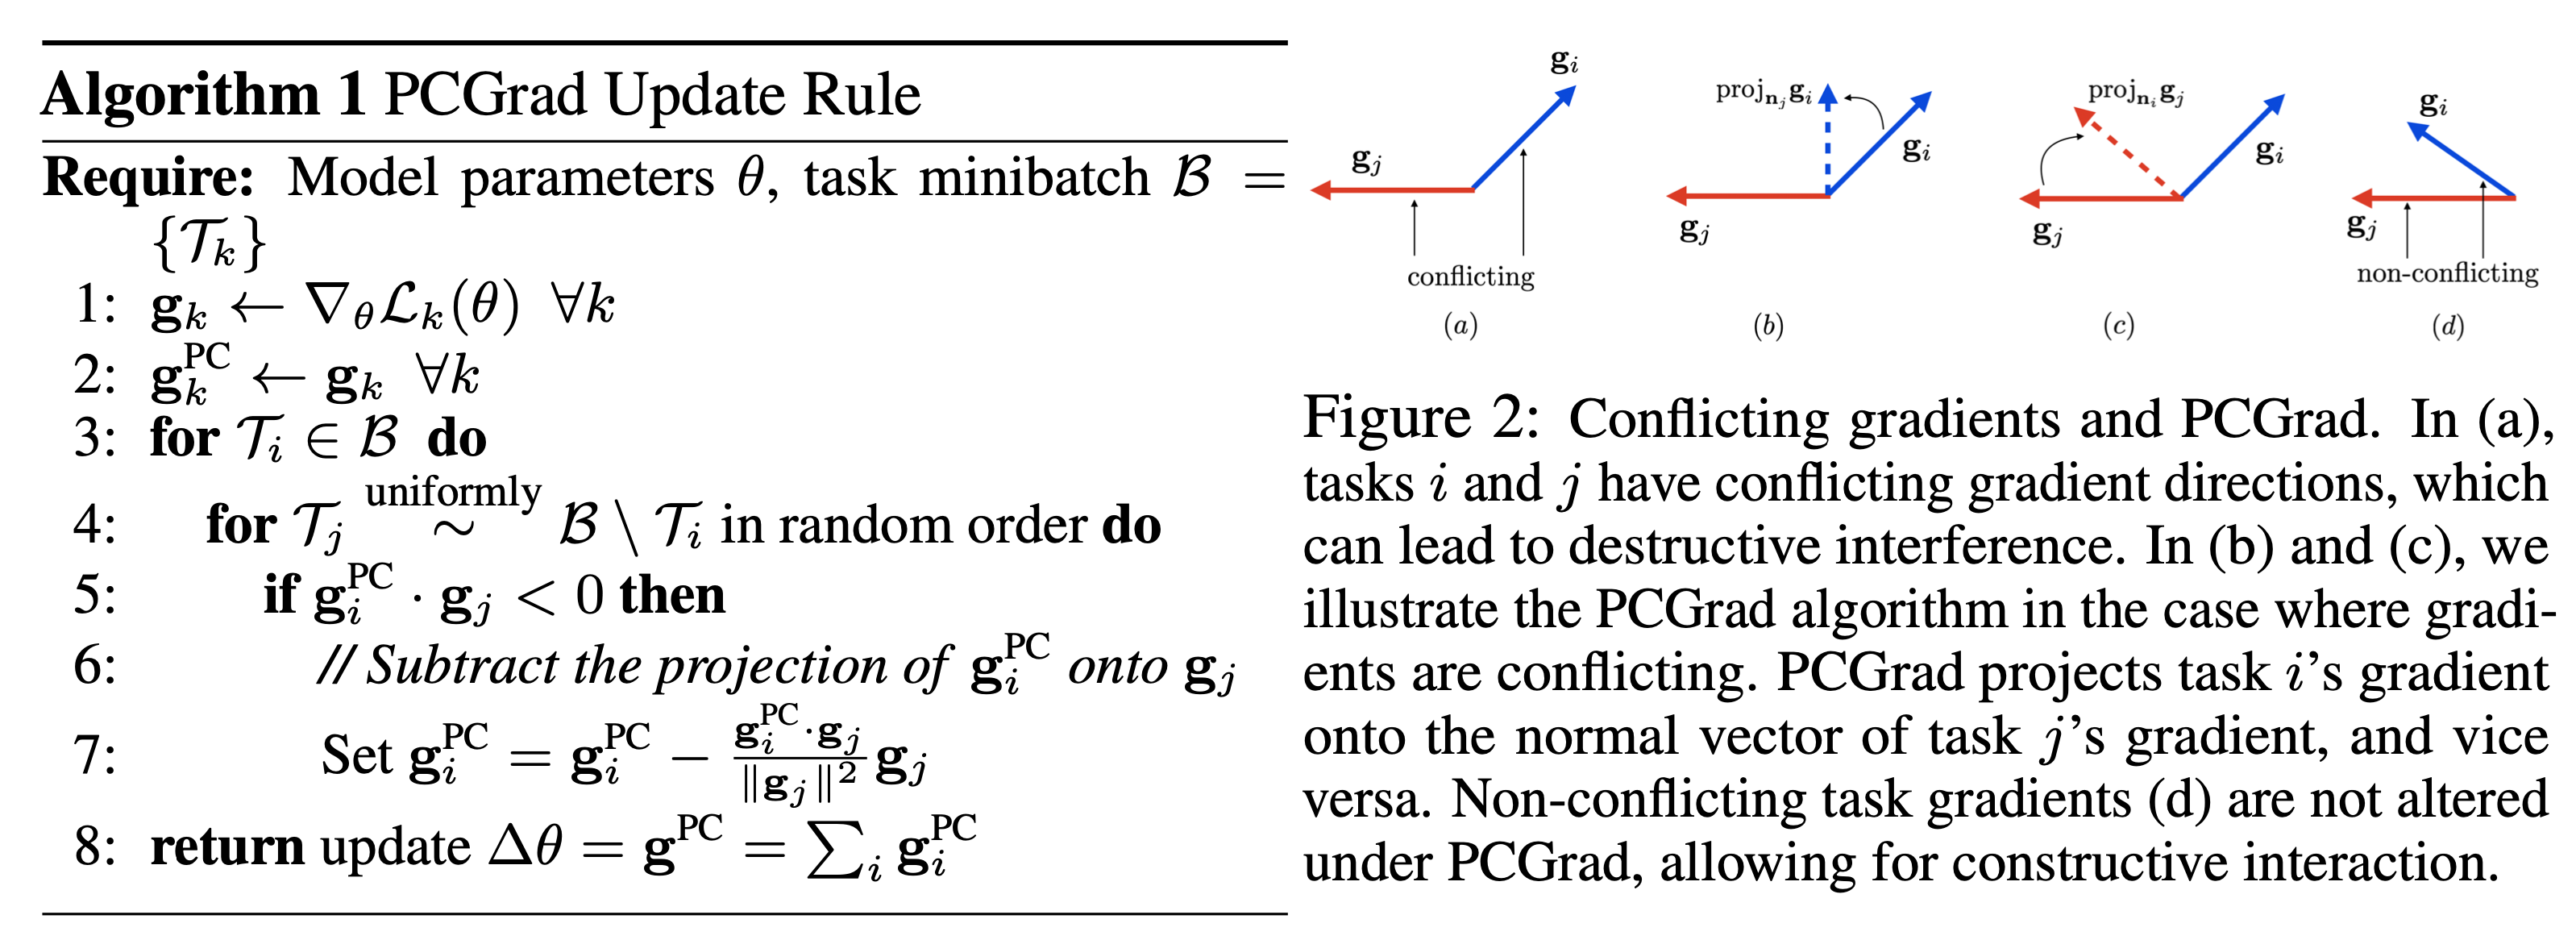
\includegraphics[width=1\textwidth]{assets/grad_angle_solution.png}
	\end{figure}
	\href{https://arxiv.org/abs/2001.06782}{\color {blue} Yu et al. Gradient Surgery for Multi-Task Learning. 2020}
\end{frame}

\begin{frame}
	\frametitle{Гипотеза 1: стандартная}
	\begin{itemize}
		\item Рассмотрим задачу $i$-ую классификации последовательности $T_i = \{p_i(x), p_i(y | x), H_i, L_i\}$, где $p_i(x), p_i(y|x)$ - распред. входов, меток
		\item Функция потерь $L_i(p, y) = - \sum_{c}^{C_{i}} \delta_{c, y} \log p_c$ (кросс-энтропия)
		\item Зафиксируем гипотезу для общих слоёв $E$ - стек энкодеров Трансформера
		\item $\dim E$ - размерность выходных векторов; $C_i = {1, 2, ..., K_i}, K_i$ - число классов
		\item Прямой проход по нейронной сети для задачи $i: F_i(\operatorname{seq}) = H_i \circ E_{\operatorname{CLS}} \circ \operatorname{seq}$
	\end{itemize}

	\textbf{Гипотеза}

	$H_i^1 = \opreatorname{softmax} \circ \operatoname{linear}_i$

	\begin{itemize}
		\item $\operatorname{linear}_i(x) = W_i[1; x]; \operatorname{linear}_i : R ^ {dim E} \rightarrow R ^ {K_i}$
		\item $\operatorname{softmax}(x)_i = \frac{\exp(x_i)}{\sum_{k = 1}^{K_i} \exp(x_k)}; \operatorname{softmax} : R ^ {M} \rightarrow R ^ {M}$
	\end{itemize}
\end{frame}

\begin{frame}
	\frametitle{Гипотеза 2: стек линейных слоёв}
	\begin{itemize}
		\item Рассмотрим задачу $i$-ую классификации последовательности $T_i = \{p_i(x), p_i(y | x), H_i, L_i\}$, где $p_i(x), p_i(y|x)$ - распред. входов, меток
		\item Функция потерь $L_i(p, y) = - \sum_{c}^{C_{i}} \delta_{c, y} \log p_c$ (кросс-энтропия)
		\item Зафиксируем гипотезу для общих слоёв $E$ - стек энкодеров Трансформера
		\item $\dim E$ - размерность выходных векторов; $C_i = {1, 2, ..., K_i}, K_i$ - число классов
		\item Прямой проход по нейронной сети для задачи $i: F_i(\operatorname{seq}) = H_i \circ E_{\operatorname{CLS}} \circ \operatorname{seq}$
	\end{itemize}

	\textbf{Гипотеза}

	$H_i^2 = \opreatorname{softmax} \circ \operatoname{linear}_{i, L}  \circ ... \circ \operatoname{relu} \circ \operatoname{linear}_{i, 2} \circ \operatoname{relu} \circ \operatoname{linear}_{i, 1}$
	
	\begin{itemize}
		\item $\operatorname{linear}_{i, j}(x) = W_{i, j}[1; x]$
		\item $\operatorname{linear}_{i, 1} : R ^ {\dim E} \rightarrow R ^ {d}$
		\item $\operatorname{linear}_{i, l} : R ^ {d} \rightarrow R ^ {d} \text{ } \forall l = \overline{2, (L-1)}$
		\item $\operatorname{linear}_{i, L} : R ^ {d} \rightarrow R ^ {K_i}$
		\item $\operatorname{softmax}(x)_i = \frac{\exp(x_i)}{\sum_{k = 1}^{K_i} \exp(x_k)}; \operatorname{softmax} : R ^ {M} \rightarrow R ^ {M}$
	\end{itemize}
\end{frame}

\begin{frame}
	\frametitle{Гипотеза 3: накинем вниманий}
	\begin{itemize}
		\item Рассмотрим задачу $i$-ую классификации последовательности $T_i = \{p_i(x), p_i(y | x), H_i, L_i\}$, где $p_i(x), p_i(y|x)$ - распред. входов, меток
		\item Функция потерь $L_i(p, y) = - \sum_{c}^{C_{i}} \delta_{c, y} \log p_c$ (кросс-энтропия)
		\item Зафиксируем гипотезу для общих слоёв $E$ - стек энкодеров Трансформера
		\item $\dim E$ - размерность выходных векторов; $C_i = {1, 2, ..., K_i}, K_i$ - число классов
		\item Прямой проход по нейронной сети для задачи $i: F_i(\operatorname{seq}) = H_i \circ E_{\operatorname{CLS}} \circ \operatorname{seq}$
	\end{itemize}

	\textbf{Гипотеза}

	$H_i^3 = H_{i}^{h} \circ \operatorname{subEncoder}_{i}$
	\begin{itemize}
		\item $\operatoname{subEncoder}_{i} = \operatorname{MHSA}_{i, M} \circ ... \circ \operatorname{MHSA}_{i, 2} \circ \operatorname{MHSA}_{i, 1}$
		\item $\operatorname{MHSA}_{i, m} = \operatorname{concat}(\operatorname{head}_1^{(i)}(X), ..., \operatorname{head}_h^{(i)}(X))W_{O}^{(i)}$
		\item $\operatorname{head}^{(i)}(X) = \operatorname{softmax} \Bigg ( \frac{Q(X)K(X)^T}{\sqrt{d_h}} \Bigg ) V(X)$
		\item $Q(X) = X W_{Q}^{(i)}, K(X) = X W_{K}^{(i)}, V(X) = X W_{V}^{(i)}$
	\end{itemize}
\end{frame}

\begin{frame}
	\frametitle{Что успел сделать по этому пункту}
	\begin{itemize}
		\item Первая гипотеза точно работает, с ней были основные эксперименты на данный момент
		\item Первая гипотеза начинает плохо работать, если много задач / сложные задачи
		\item $\Rightarrow$ первая гипотеза не достаточно выразительна
		\item Вторая гипотеза работает (сходится)
		\item Вторая гипотеза работает не хуже первой
		\item Третья гипотеза нормально работала в однозадачной модели
		\item Продолжаю активно тестировать данные гипотезы
	\end{itemize}
\end{frame}

\subsection{Russian SuperGLUE}

\begin{frame}
	\frametitle{Текущая таблица лидеров}
	\begin{figure}
	    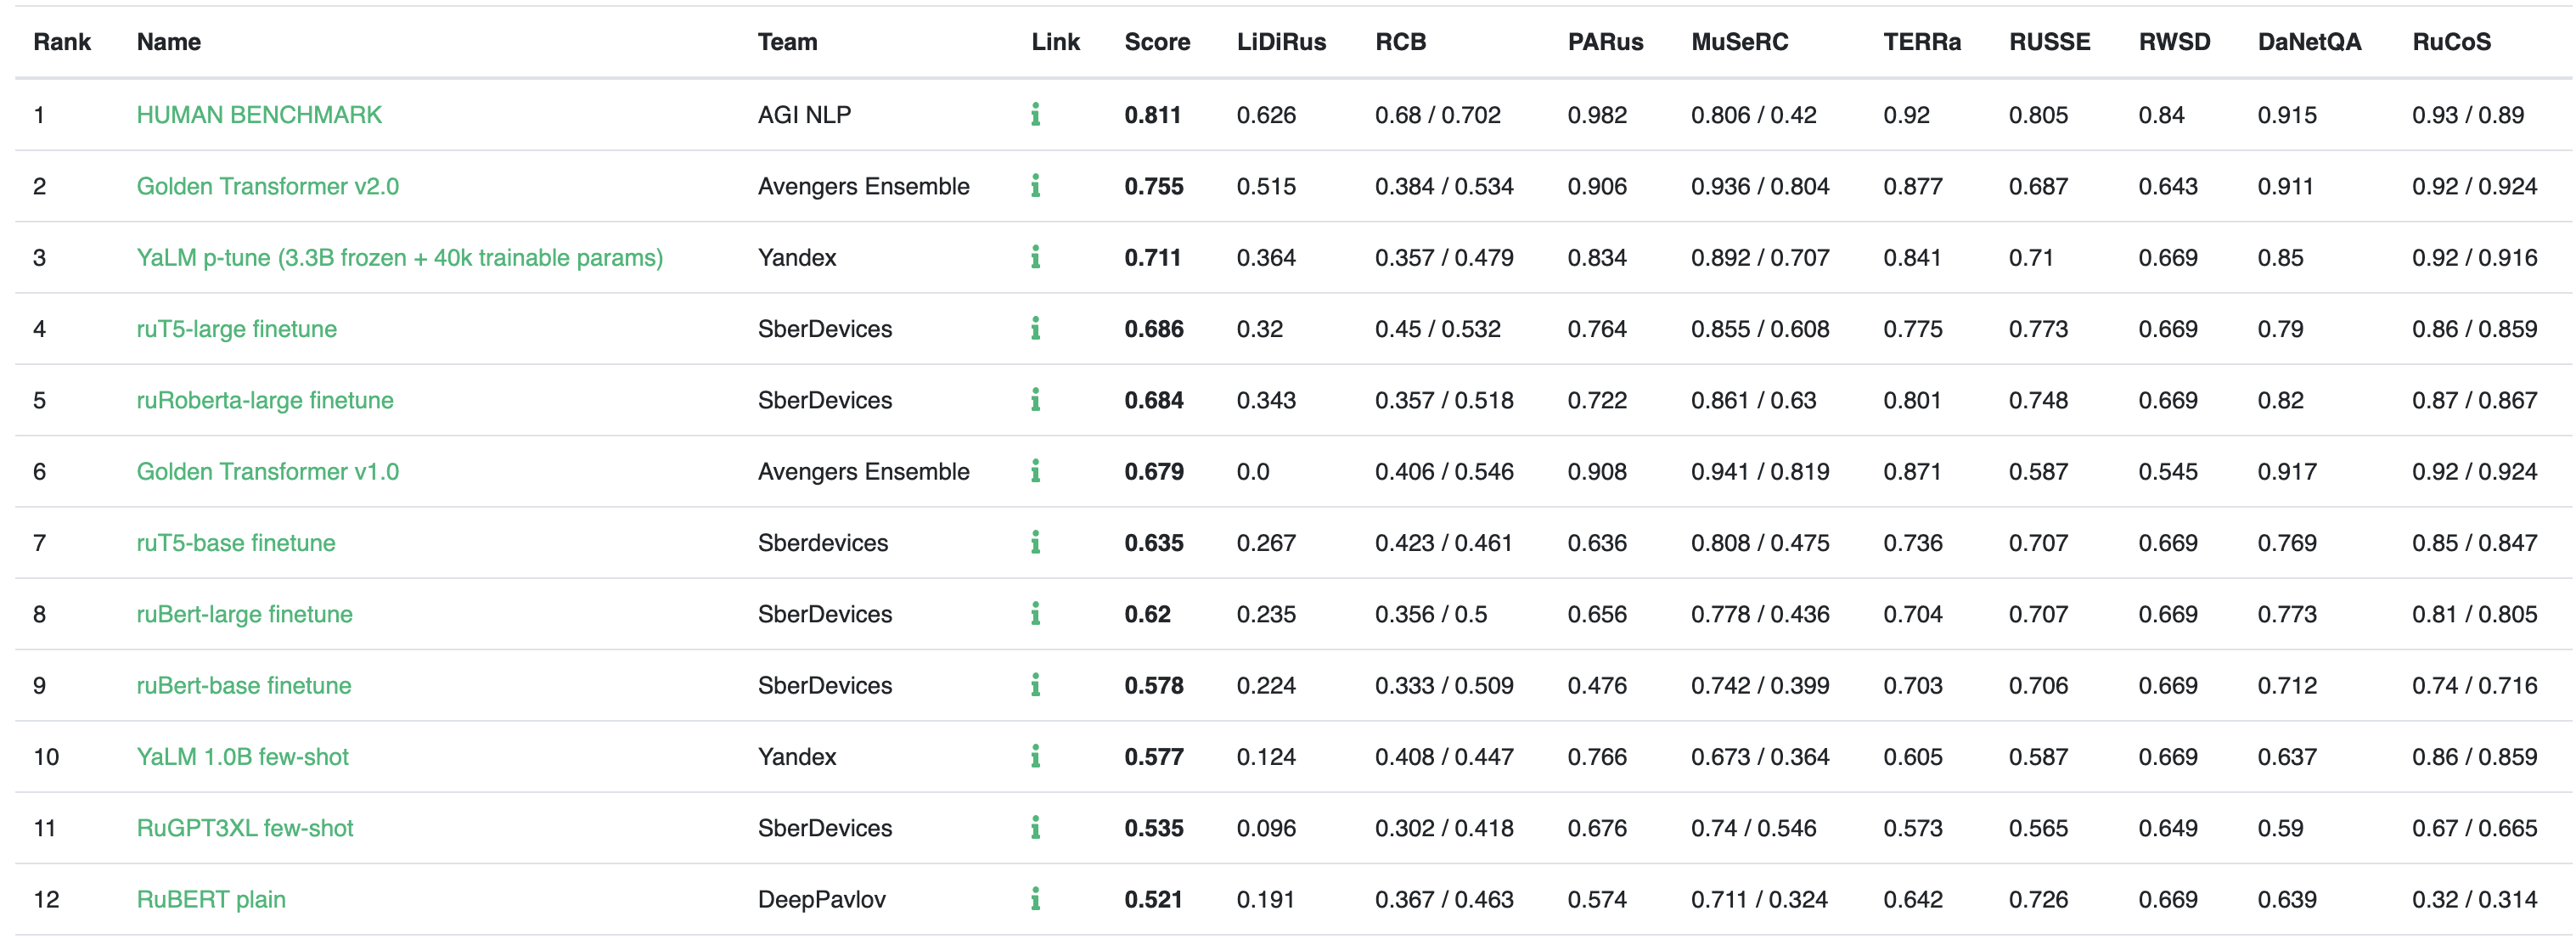
\includegraphics[width=1\textwidth]{assets/rsg_lb.png}
	\end{figure}
\end{frame}

\begin{frame}
	\frametitle{Материалы / источники}
	\begin{itemize}
		\item \href{https://cs330.stanford.edu/}{\color {blue} Стэнфордский курс CS 330: Deep Multi-Task and Meta Learning}
		\item \href{https://ruder.io/multi-task/}{\color {blue} An Overview of Multi-Task Learning in Deep Neural Networks}
		\item \href{https://arxiv.org/abs/2001.06782}{\color {blue} Yu et al. Gradient Surgery for Multi-Task Learning. 2020}
		\item \href{https://arxiv.org/abs/2009.00909}{\color {blue} A Survey on Negative Transfer. 2021}
	\end{itemize}
\end{frame}
\end{document}